\documentclass{article}
\usepackage{graphicx} % Required for inserting images
\usepackage{multicol}
\usepackage{cite}
\usepackage{amsmath}
\usepackage{amssymb}
\usepackage{subcaption}
\usepackage{hyperref}
\usepackage{ragged2e} 
\usepackage{caption}



\title{Yapay Zeka ve İnsanlığın Geleceği}
\author{Murathan Sevinç}
\date{}

\begin{document}
\begin{figure}
\centering
  
\includegraphics[width=7cm]{ksbu.jpg}
\end{figure}
\title{Yapay Zeka ve İnsanlığın Geleceği}
\author{Murathan SEVİNÇ}
\maketitle
\begin{center}
    \vfill
    \textbf{Bilgisayar Mühendisliği}\\
    \textbf{\date{Mayıs 2024}}
\end{center}

\maketitle




\newpage



\section{Giriş}
\vspace{15pt}

\begin{multicols}{2}
Toplum yapısındaki değişimlerde sanayi devrimlerinin etkisi büyüktür.Her yeni sanayi devrimi ile birlikte döneme özel toplum yapıları ortaya çıktığı söylenebilir. Kırda çalışanların kentlere akması, kentlerin büyümesi; kentlere özgü yeni
hizmetlerin ve işlerin ortaya çıkması, sosyal ve ekonomik ilişkilerin farklılaşması
gibi bir dizi birbirine bağlı süreçle değişim devam eder. Buradan çıkarılabilecek
sonuç, değişimin her yeni düzen için en temel gereklilik olduğudur. Bu gereklilik Mevlana’nın “Dün dünde kaldı cancağızım, bugün yeni şeyler söylemek lazım” sözüyle desteklenebilir. Bu değişimlere bağlı olarak, bireylerin de farklı özellikler
edinmesi ve değişikliklere ayak uydurması kaçınılmazdır.
\vspace{10pt}

İçinde bulunduğumuz yüzyılda Dördüncü Sanayi Devrimi’ni (Endüstri 4.0) yaşıyoruz. ‘Bilgi’, bu sanayi devriminde işletme düzeyinden öte, ülke düzeyinde
rekabet gücünü artıran en önemli kaynak olarak görülmektedir. Bilginin en alt
seviyede veriden elde edildiği gerçeği, aslında rekabetin veri zenginliğine indirgenebileceğini de göstermektedir. Sahip olunan verilerden anlamlı bilgiler elde edilmesi, bilginin en etkin şekilde depolanıp saklanması ve ihtiyaç duyulduğunda hızlı bir şekilde kullanılabilmesi, yeni yöntemler geliştirilmesini gerektirmektedir. Bunun yolu ise, hızlı çalışma kabiliyetine sahip olan ve ayrıca
insan beyninin çalışma anlayışı ile olabildiğince bütünleştirilmiş teknolojilerin
kullanımından geçmektedir. Bu teknolojilerden en öne çıkanı ise, hiç şüphesiz,
aslında yıllardır önemli bir araştırma alanı olarak kabul edilen, ancak son yıllarda oldukça popülerleşen Yapay Zekâ’dır.

Yapay Zekâ’nın doğru bir şekilde tanımlanabilmesi ve anlaşılabilmesi, teknolojik
ve bilimsel gelişmelerin artması ve etkinliği açısından büyük önem taşımaktadır.
Bir başka deyişle, mevzubahis toplumsal değişimin temel unsurlarından olan
Yapay Zekâ kelimesinin, kavramının veya teknolojisinin anlamını ve neyi ifade
ettiğini çok iyi idrak etmek gerekmektedir. Konuyu derinlemesine kavrayabilmek için, öncelikle; “Zekâ nedir? Eş anlamlısı olarak bilinen ‘akıl’ kavramının kullanımı doğru mudur? Yapay Zekâ var, ama neden Yapay Akıl yok?” gibi sorulara cevap
aramak gerekir. Zekâ kelimesinin sözlük anlamının, Türk Dil Kurumu (TDK) tarafından; “İnsanın düşünme, akıl yürütme, nesnel gerçekleri algılama, kavrama, yargılama ve sonuç çıkarma yeteneklerinin tümü” olarak verildiği görülmektedir. Akıl
kelimesinin ise TDK sözlüğünde : “Düşünme, anlama ve kavrama gücü, us”, “Öğüt,
salık verilen yol”, ”Düşünce, kanı”, “Bellek” olarak tanımlandığı görülmektedir.
Kavramlar arasındaki çizgi keskin hatlarla belirlenemediği için, bu durum farklı
anlaşılmalara, yorumlara ve yanılgılara sebebiyet verebilmektedir. Misalen; ‘akıl’
ve ‘akıllı’ kavramları gerek bilimsel hayatta gerekse de sosyal hayatta, robotların, makinelerin, ev gereçlerinin özelliklerini belirtmede vazgeçilmez bir sıfat
olmuştur. Oysa bu kavramlar sadece insanlara özgüdür. Akıl, sadece insanlara
özgü olduğu ve taklit edilemez olduğu için, aklını kullanabilen insanlara ‘akıllı’
denilmektedir. Zekâsını kullanarak ‘zeki’, aklını zekâsıyla birleştirerek akıllı olabilen, insandır. Bu bağlamda; sistemlerin, makinelerin, robotların, ev gereçlerinin gerçekten ‘akıllı’ olarak nitelendirilmesi aslında uygun değildir. Yapay Zekâ
algoritmalarını kullanarak, kural tabanına bağlı kalarak, kendilerine verilen görevleri yerine getirebilen sistemler ise ‘zeki’ olarak nitelendirilebilir. Zekânın ve
zekiliğin taklit edilebilmesi sayesinde Yapay Zekâ kavramı ortaya çıkmıştır. Literatürde, Yapay Zekâ için verilen pek çok tanım bulunmaktadır. En kabul gören
tanımlarından birinde Yapay Zekâ; insan tarafından yapıldığında ‘zekâ’ olarak
adlandırılan davranışların, makine tarafından da yapılması olarak tarif edilmektedir. En yalın haliyle, sözlük tanımı olarak Yapay Zekâ; ‘bir bilgisayarın veya bilgisayar kontrolündeki bir robotun çeşitli faaliyetleri, zeki canlılara benzer şekilde yerine getirme kabiliyeti’ olarak tanımlanabilir. Başka bir deyişle, bir sistemin harici verileri doğru bir şekilde yorumlayabilme, bu verilerden öğrenebilme ve bu öğrenmeleri
esnek adaptasyon yoluyla belirli hedeflere ve görevlere ulaşmak için kullanma yeteneğine Yapay Zekâ adı verilebilir. Yapay Zekâ, günümüzde; insanların entelektüel özelliklerine, davranışlarına, geçmiş deneyimlerden öğrenme, algılama
yetenekleri ve tahmin yapma ve belirli durumun anlamını belirleme yeteneklerine sahip çeşitli robotlar geliştirme için kullanılmaktadır. Görüntü tanıma ve
sürücüsüz otomobiller gibi birçok teknoloji Yapay Zekâ alanındaki ilerlemeler
sayesinde mümkün hale gelmiştir.
 Ülke ve/veya kurumsal varlığı sürdürebilmek, ilgili
kurum ya da kuruluşların bu değişim sürecini yönetebilmeleri ile doğru orantılı
hale gelmiştir. Çünkü değişimin önü alınamaz hale gelmiştir. Sürekli dile getirilen “değişmeyen tek şey değişimin kendisidir” söylemi çok açık olarak kendisini göstermektedir. Günümüz itibari ile dünya öyle bir noktaya gelmiştir ki bu
dönüşüm sürecine ayak uydurmakta zorlananların gelecekte büyük sorunlar ile
karşı karşıya kalacaklarında, diğerleri ile rekabet edemeyeceklerinde, hatta varlıklarını bile sürdüremeyeceklerinde herhangi bir şüphe bulunmamaktadır. Global dünyanın aktif aktörleri, başkalarının kaynaklarını kendi ülke ya da kurum
menfaatleri doğrultusunda kullanmak için diğerlerini ezip geçmekten çekinmeyecektir.

\vspace{10pt}
Bu makalenin amacı endüstriyel ve sosyal dönüşümün yanı sıra yapay zekâ teknolojisinin toplum ve insanlığın bugün ve yarınında nasıl etkiler oluşturacağına
dikkatleri çekmek ve geleceğe doğru bir bakış sunmaktır.

\newpage
\section{Geçmişten Günümüze Yapay Zeka}
Yapay Zekâ’nın en eski izine 1884 yılında Charles Babbage tarafından, bazı zeki
davranışlar göstermesini istediği birtakım makineler üzerinde yapılan deneylerde rastlanmaktadır. Bu makinelerin zekileştirilebilmesi için uzun soluklu çalışmalar yapılmıştır. İnsan kadar asla zeki olamayacağı üzerinde hemfikir olunan
bu makineler üzerindeki çalışmalar sürdürülerek, Yapay Zekâ’nın etkinliğini
artıran bilgisayarların altyapısı hazırlanmıştır. “Mind: A Quarterly Reviews of Psychology and Philosophy” dergisinde yayınlanan Alan Turing’in makalesinin giriş
cümlesindeki; “I propose a question: Can Machine think!” sorusu ile 1950’de bir
makinenin zeki olup olmadığına karar verme olanağı tanıyan bir test ortaya konulmuştur. Temel kuralı tartışmalı olmakla birlikte bu test, bu dönemden itibaren bilgisayarların zekâsına verilen önemi gayet iyi göstermektedir. 1959 yılında
Atatürk Üniversitesi Halk Konferansları kapsamında konuşan 

ordinaryüs Prof.
Dr. Cahit Arf da Alan Turing ile benzer bir soruyu sormuş, hatta biraz daha ileri
giderek, makinelerin nasıl düşünülebilecekleri detayına da değinmiştir.

 \vspace{20pt}
 
\begin{minipage}{\linewidth}
    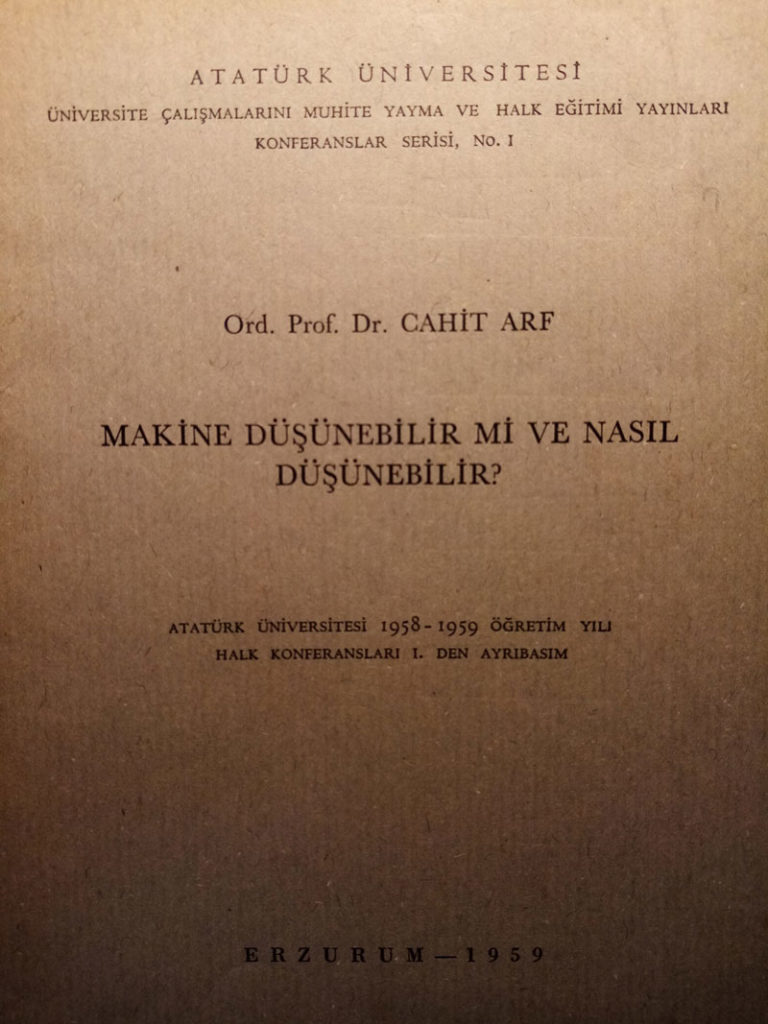
\includegraphics[width=1\linewidth]{carf.jpeg} 
    \label{fig:Şekil tekrar}
\end{minipage}

\centering {\hspace*{1pt} Prof. Dr. Cahit Arf \hspace*{1pt} “Makine Düşünebilir mi ve Nasıl \hspace*{1pt} Düşünebilir?” başlıklı kitabı \cite{ref1}}
\end{multicols}
\begin{multicols}{2}

Yapay Zekâ terimi literatürde ilk kez 1956 yılında Dartmouth’ta düzenlenen ve
altı farklı bilim dalından yedi bilim insanını bir araya getiren bir konferans sonrasında ortaya koyulan; “The Dartmouth Summer Research Project on Artificial Intelligence” başlıklı araştırma raporunda kullanılmıştır. Bu konferansta; J. McCarthy, M. Minsky (MIT Yapay Zekâ Laboratuvarı kurucusu), C. Shannon, A. Newell
(Amerikan Yapay Zekâ Derneği’nin ilk başkanı) ve H. Simon, zekâ ile donatılmış
bilgisayar programlarının gerçekleştirme olasılığını araştırmayı önermişlerdir.
İlk Yapay Zekâ programları (bir mantık teoremleri uygulayıcısı, Logic Theorist
ve bir satranç oyunu programı; her ikisi de Newell ve Simon’a aittir) ve LISP
(Yapay Zekâ programlama dili) de yine aynı dönemde ortaya çıkmıştır.
\newpage
1960’lar Yapay Zekâ alanında aşırı iyimserliğin hüküm sürdüğü ve bilim insanlarının zeki bilgisayar yapımı rüyaları görmeye başladığı yıllardır ve önceki on yıla
göre kıyaslandığında, üretkenliğin çok olmadığı anlaşılmaktadır. Çalışmaların
genellikle bilgisayarlara veriler yükleme şeklinde sürdürüldüğü izlenmektedir.
Bu durgunluk döneminin ardından, 1970’li yılların özellikle ilk yarısı Yapay Zekâ
alanında artık önüne geçilemeyecek adımların atıldığı ve gelişmelerin yaşandığı
yıllar olarak kayda geçmiştir. Yapay Zekâ uzmanları bu dönemde özellikle hastalık teşhis sistemleri ve benzeri sistemler geliştirerek, bugün heyecanla sonuçları
kestirilmeye çalışılan, uzun ve heyecanlı bir maceranın temellerini atmışlardır.
Dil ve psikoloji gibi diğer bilim alanlarında da Yapay Zekâ uzmanlığından faydalanılmasının mümkün olduğunun ortaya çıkmasıyla, ilgili çalışmalar geniş bir
alana yayılarak devam etmiştir.

İçinde bulunduğumuz dönemde ise, Yapay Zekâ; laboratuvarların dışına çıkarak
toplumun gerçek ihtiyaçları için ve insanlığın yaşam kalitesinin artırılması için
uyarlanmaktadır. Daha önce geleneksel işlem metotları ile ihtiyaçları karşılanan
kullanıcılar, bugün ekonomik olarak daha uygun maliyetli yazılımlara ve zeki araçlara ulaşabilmektedir. Bu sayede, Yapay Zekâ günlük yaşamda geniş kullanım alanları bulmaktadır. Yapay Zekâ uygulamalarının hayatımızın her alanında
kullanılabileceği, en önemli konulardan birinin ise ‘tahminleme’ olduğu kabul
edilmektedir. Yapay Zekâ’nın en çok uygulama alanı bulduğu alanlardan bir
diğeri de robotik uygulamalarıdır. 

Endüstriyel uygulamaların yanı sıra insansı
robotların hizmet sektöründe kullanımı giderek yaygınlaşmaktadır. Yapay Zekâ
ile donatıldığı iddia edilen robot Sophia’ya Suudi Arabistan’da vatandaşlık verilmesi, Çin’de Xiao Yi ismi verilen bir robotun tıp alanında yapılan bir sınavı
başarı ile geçmesi, IBM’in Watson isimli doğal dilde sorulan sorulara cevap vermek için tasarladığı Yapay Zekâ programının bilgi yarışmalarına dahi yarışmacı
olarak katılması, haberlere konu olan ilgi çekici başlıklar arasına girmiştir.


\vspace{10pt}
\begin{minipage}{\linewidth}
    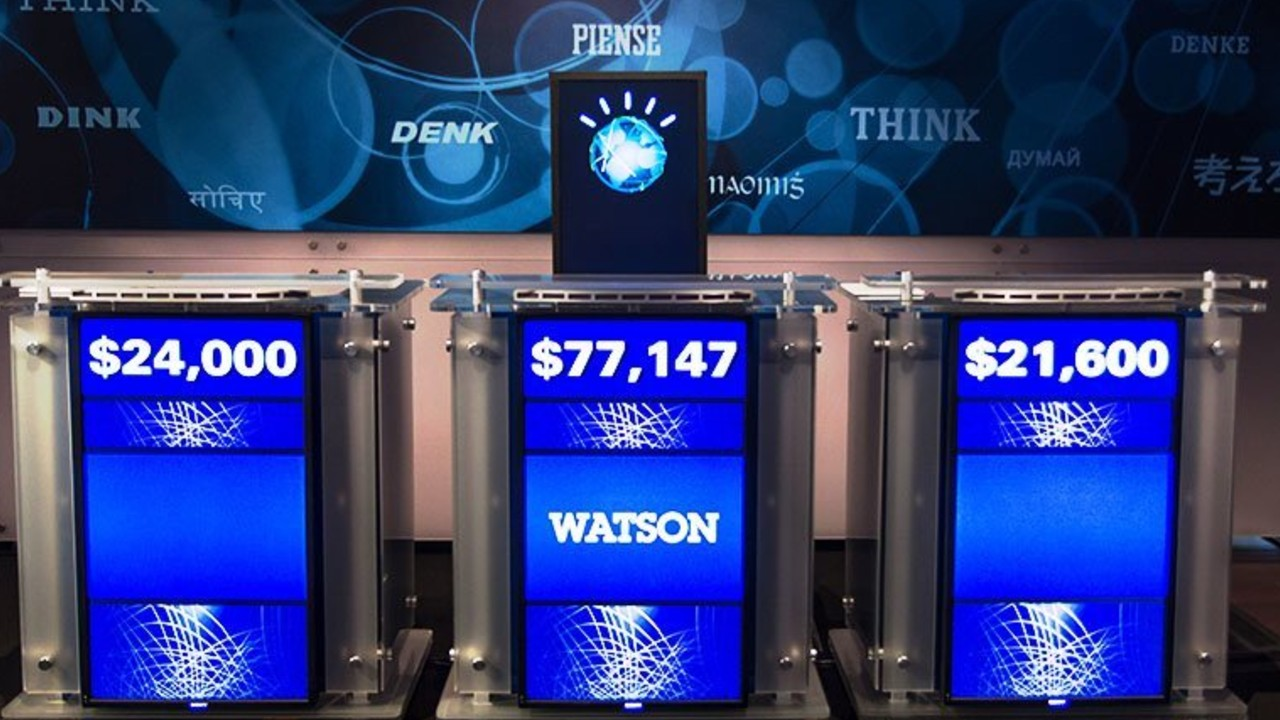
\includegraphics[width=1\linewidth]{n.jpeg} 
    \label{fig:Şekil tekrar}
\end{minipage}

\centering {\hspace*{1pt} IBM tarafından tasarlanan Watson \cite{ref2}}

\end{multicols}

\newpage
\begin{multicols}{2}

Dördüncü Sanayi Devrimi’ni doğru anlayabilmek ve doğru işler
yapabilmek için veri, veri dili, veri akışkanlığı ve veri kalitesi çok önemli hale gelmiştir. Veri olmadan, bu aşamada Yapay Zekâ uygulaması gerçekleştirmek neredeyse mümkün değildir. Artırılmış gerçeklik uygulamaları buna iyi bir örnektir. Artırılmış gerçeklik, gerçek dünya görüntüsünün üzerine sanal dünyaların, sanal imajların, sanal bilgilerin entegre edilmesi şeklinde karşılık göstermektedir. Veri
olmadan işlevsellik elde edilemez. Yapay Zekâ’nın etkin çalışabilmesi için gerekli veri elde edilmiş olmalıdır. Sığ Yapay Zekâ olarak nitelendirilen ve 1980’li yıllardan bu yana geliştirilmeye devam edilen robotların ve uygulamaların yerini,
artık Yaygın Yapay Zekâ almaktadır. Sonrasında ise, Süper Yapay Zekâ olarak
adlandırılabilecek ve insanoğlunun bugün tahmin dahi edemeyeceği gelişmeler
ve teknolojiler ile karşı karşıya kalınabilecektir.

Hızla gelişen Yapay Zekâ’ya dayalı teknolojiler nedeniyle, dünyadaki küresel
oyuncular ve kimi ülkeler, bu teknolojilerin ve dijitalleşmenin sunacağı fırsatları ekonomik değere dönüştürmek için stratejiler geliştirmeye çalışmaktadır. Bu
alanın önemli oyuncularının ABD, Çin, Almanya ve Japonya olacağı tahmin edilmektedir. Google, IBM, Samsung, Yahoo, Intel, Apple gibi şirketler Yapay Zekâ
alanına devasa yatırımlar yapmaktadır. İnsanoğlu hakkında en iyi ve en fazla
bilgiye sahip olan şirketlerden birinin Google olduğu düşünülmektedir. Google,
Yapay Zekâ konusu ile ilgilenen, sadece birkaç ay önce kurulmuş start-up şirketlerini bile satın alarak, bu konudaki yatırımlarını artırmaktadır. Büyük veri toplama yeteneği son derece gelişen Çin’in Yapay Zekâ konusundaki yatırımları ve
çalışmaları da dikkat çekicidir. Çin’in bu konuya verdiği önem, akademik alanda
değerlendirildiğinde de ortaya çıkmaktadır. Literatürde en çok atıf yapılan Yapay Zekâ makalelerin sayısı ve bu alana katkı yapan yazar sayısı bakımından Çin
birinci konumdadır. Patent sayılarında da durum aynıdır. Yapay Zekâ alanında
araştırma yapan, bilgi ve know-how üreterek teknoloji geliştiren ve bunlara yatırım yapan ülkelerin ve toplumların gelecekte kazançlı çıkacağı aşikârdır.
\end{multicols}
\begin{figure}[h]
\centering
  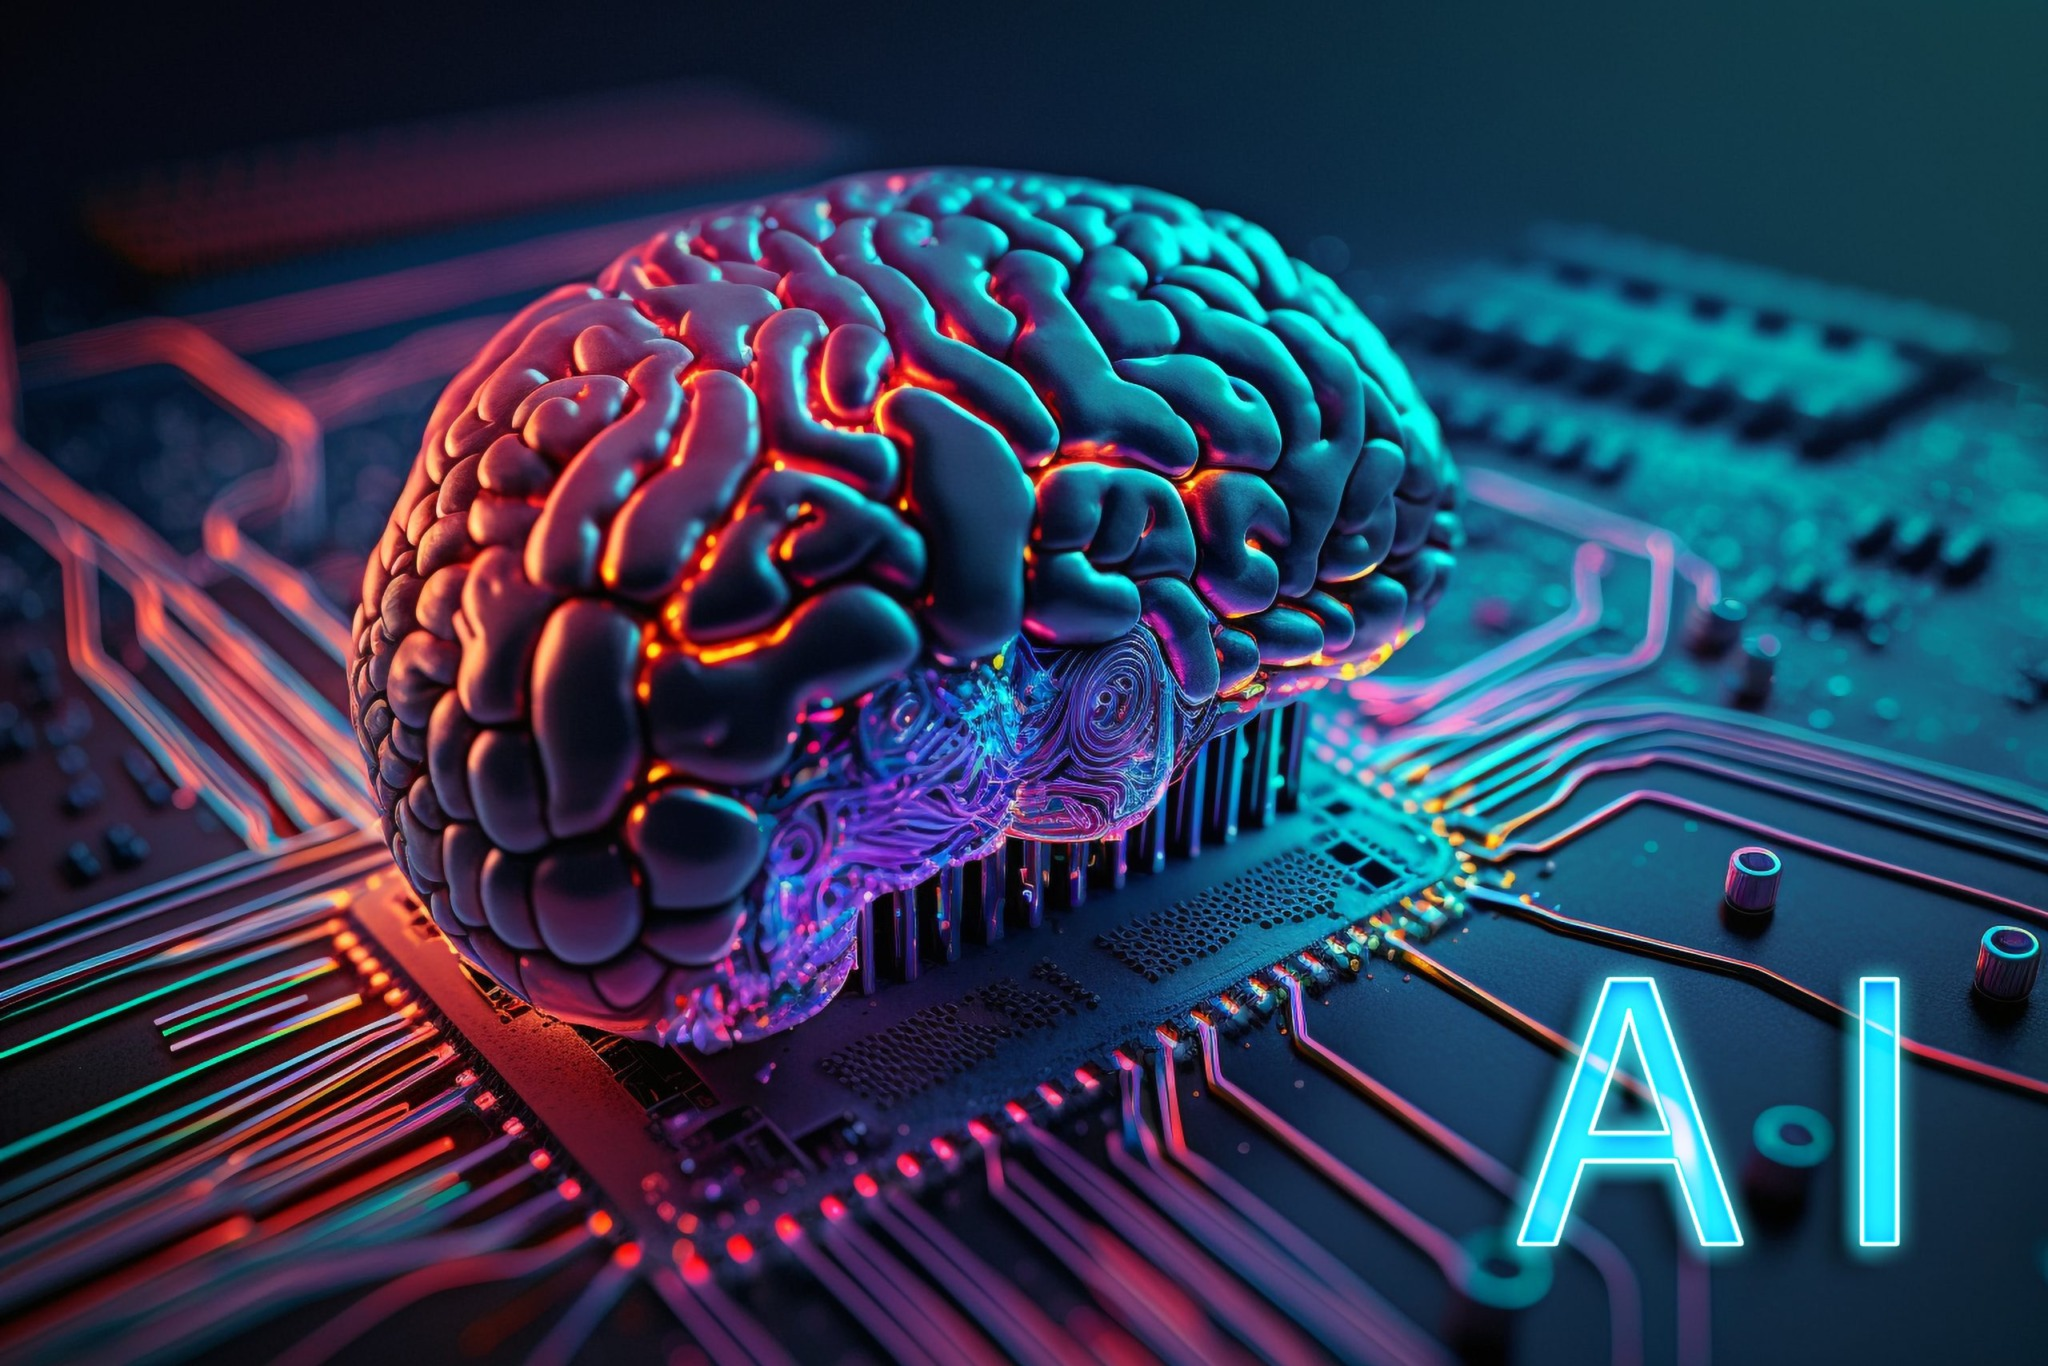
\includegraphics[width=8cm, height=4cm]{1.jpeg}
  \caption{\cite{ref3}}
\end{figure}
\newpage
\section{Yapay Zekâ’nın İnsanlık Üzerine Etkileri}
\begin{multicols}{2}
Yapay Zekâ kavramı, kimi zaman, insan müdahalesi olmadan öğrenebilen, kendi kendine karar verebilen ve öğrendiklerini uygulayabilen bir algoritma olarak
da tanımlana gelmektedir. Hatırlanacağı üzere, “The Social Network” filmi, Facebook’un İcra Kurulu Başkanı Mark Zuckerberg’in sahip olduğu sosyal platformunun ortaya çıkış öyküsünü ele alır. Filmde geçen en dikkat çekici cümle, Zuckerberg’in kurmak istediği platform için bilgisayar mühendisi bir arkadaşından
yardım isterken kullandığı; “Bana bir algoritma lazım” cümlesidir. Yapay Zekâ’ya
yeteneğini kazandırıp yükselmesini sağlayan en önemli araç, aslında insan davranışlarına yakın sonuçlar üretebilen güvenilir algoritmalardır. 

Yapay Zekâ’nın amaçlarından birinin, makineleri daha zeki ve faydalı hale getirmek olduğu söylenebilir. Burada hangi davranışların daha zeki olarak değerlendirildiği sorusu ortaya çıkmaktadır. Bir sistemin veya robotun, zeki olarak
nitelendirilebilmesi için; tecrübelerden öğrenme ve anlama, karışık ve zıt mesajlardan anlam çıkarma, yeni bir duruma başarılı ve çabuk bir şekilde cevap
verme, problemlerin çözümünde muhakeme yeteneğini kullanma, bilgiyi anlama ve kullanma, alışık olunmayan ve şaşırtıcı durumların üstesinden gelebilme
yeteneği vb. gibi özelliklere sahip olması gerekmektedir.

Günümüzde Yapay Zekâ’nın öne çıkan iki itici gücünün; Derin Öğrenme (Deep
Learning) ve Makine Öğrenmesi (Machine Learning) olduğu göz önünde bulundurulduğunda, zekiliğin temel özelliğinin, öğrenme yeteneği olduğu rahatlıkla
anlaşılabilir. Bu nedenledir ki Yapay Zekâ ve teknolojileri, bu terim ilk duyulduğunda insanların aklına gelen robotlar gibi sadece maddi bir varlıktan ibaret olmayıp, günümüzde öğrenme yeteneğine sahip olan ve yeni durumlar karşısında
kendi kendine kararlar alarak aksiyon gösterebilen sistemler olarak karşımıza
çıkmaktadır.

Günümüzde Yapay Zekâ tabanlı uygulamalar hastaların ve yaşlıların sağlık koşullarının ve yaşam kalitelerinin iyileştirilmesine yardımcı olmaktadır. Yapay
Zekâ’nın sağlık hizmetlerindeki başlıca uygulamaları arasında, tıbbi gelişmelerin izlenmesi, kronik hastalıkların tedavisi, hastalıkların teşhisi ve cerrahi destek
bulunmaktadır. Yapay Zekâ tabanlı ev sağlığı yardımcılarının sayısının önümüzdeki 10 yıl içinde %38 oranında artacağı ve kişiselleştirilmiş rehabilitasyon ve ev
içi terapi nedeniyle hastanede kalış süresinin azalacağı öngörülmektedir. 2012-
2017 yılları arasında sağlık alanındaki Yapay Zekâ çalışmalarına yapılan harcamaların 2 milyar dolara ulaştığı tahmin edilmektedir. Sağlık risklerini tahmin
etmek için sosyal medya madenciliği, riskli hastaları tahmin etmek için makine
öğrenmesi ve cerrahiyi desteklemek için robotik dâhil olmak üzere birçok Yapay
Zekâ tabanlı uygulama, sağlık sektöründe başarı ile kullanılmaktadır.
Yapay Zekâ, imalat sektöründe ekipmanların gerçek zamanlı bakımı ve sanal
tasarımı gibi birçok fayda sağlamıştır. Yapay Zekâ araçları ile tasarımcı bir çözümün tüm olası permütasyonlarını araştırabilmekte, hızlı bir şekilde tasarım
alternatifleri oluşturabilmekte ve bunların fizibilitesinin test edilmesini sağlayabilmektedir. Manuel olarak yapılamayacak büyüklükteki mühendislik çalışmalarının çok hızlı bir şekilde yapılması, Yapay Zekâ araçları ile mümkün hale
gelmiştir.
Yapay Zekâ’nın doğal dil işleme yeteneği, okuma yazma bilmeyen ve bilgisayar kullanamayan kişilere fayda sağlamaktadır. Yapay Zekâ, öğretmenlerin not
verme gibi tekrarlayan görevlerden kurtulmasına yardımcı olmakta ve öğretmenlerin daha fazla profesyonel çalışmaya odaklanmalarına izin vermektedir.
Yapay Zekâ araçları ile okula devam edemeyen öğrenciler de dâhil olmak üzere,
sınıfların herkese açık olması sağlanabilmektedir.

\vspace{5pt}
Günümüze değin yaşanan teknolojik gelişmeler ile Yapay Zekâ aslında adım
adım hayatımıza yerleşmiştir. Yapay Zekâ sadece kişisel hayatlarımızı etkilemekle kalmamış, iş hayatında karar alma ve paydaşların etkileşim biçim ve süreçlerini de radikal olarak değiştirmeye başlamıştır. Hangi kararların Yapay Zekâ
tarafından, hangi kararların ise insanlar tarafından alınması gerektiği ve nasıl
iş birliği içinde olunması gerektiği soruları zihinleri kurcalamaya başlamıştır.

\vspace{5pt}
Aslında, Yapay Zekâ denilince akla gelen ve artık klasikleşmiş birçok soru vardır: "Zekâ nedir? Akıl’dan farkı nedir? Yapay Zekâ nedir? Doğal Zekâ’dan farkı nedir?
Hangisi üstündür? Yapay Süper Zekâ’ya sahip sistemleri ne zaman göreceğiz?
Yapay Zekâ teknolojileri nasıl ilerleyecek? Getirdiği riskler nelerdir? Neden bu
kadar çok insan Yapay Zekâ’yı konuşuyor ve Yapay Zekâ’nın potansiyeli ve tehdidi hakkında bu kadar güçlü fikirlere sahip? Öte yandan, acaba Yapay Zekâ’ya sahip
robotlar ne kadar insansı olacaklar? İnsanlar ile birlikte yaşayabilecekler mi ve
çalışabilecekler mi? Kendilerine bir dil icat edip bir robot toplumu oluşturabilecekler mi? İnsanlar üzerinde hâkimiyet kurabilecekler mi? Ne kadar tehlikeli ya da
yararlı işlere imza atacaklar? Hayatın her aşamasındaki işleri yapabileceklerse,
insanlar ne iş yapacaklar? İnsanlar işsiz mi kalacak? Geleceğin robotları kim olacak? Makine zekâsı insan zekâsını geçebilir mi? vb."

Bu sorular katlanarak artmaya ve önümüzdeki yıllarda da cevapları aranmaya
devam edecektir. Şunu belirtmek gerekir ki, Yapay Zekâ oluşturma fikri, temelde insan hayatını kolaylaştırmayı amaçlamaktadır. Bununla birlikte, Yapay
Zekâ’nın genel olarak avantajları ve dezavantajlarını iyi irdelemek gerekir. Görevlerin yorulmadan gerçekleştirilmesini sağlaması Yapay Zekâ teknolojilerinin
en büyük avantajlarından biridir. Yapay Zekâ ile tekrar edilebilirlik çok daha
kolay hale gelir. Duyguları olmayan Yapay Zekâ teknolojileri daha doğru kararlar alabilir ve bu suretle iş verimliliğini artırabilir. Bununla birlikte, günümüzde
duygu ve hisleri de içine alan Yapay Zekâ teknolojileri geliştirilmeye çalışılmakta
olduğu düşünüldüğünde, aslında tartışmayı başka bir yere götürmek de mümkündür. Şöyle ki, bir sistemin gerçekten zeki olabilmesi için öğrenebilmesi ve
ayrıca hata da yapabilmesi gereklidir. Öğrenen sistemler eksik veya önyargılı
deneyim nedeniyle hata yapabilirler. Makine öğrenimi algoritmaları genelde
sezgiseldir ve kimi zaman başarısız olabilir. İnsanlar, bir taraftan başta robotlar
olmak üzere Yapay Zekâ teknolojilerini hata yapmayan sistemler olarak algılar
iken, diğer taraftan da öğrenebilen, hissedebilen ama hata da yapabilecek sistemler geliştirmeye çalışmaktadır. Aslında, bu dahi insanoğlunun Yapay Zekâ
konusundaki görüşlerinin hala berrak olmadığına ve otomasyondan otonomasyona geçiş sürecinin sancılı olacağına işaret etmektedir. Öte yandan, arıza riski,
Yapay Zekâ’nın en büyük dezavantajıdır. Verilerin kaybolması ile birlikte etik ve
ahlaki değerler de Yapay Zekâ alanında çok tartışılan konular arasındadır.

Burada üzerinde durulması gereken ve altı çizilmesi gereken diğer bir konu;
gerçek bir robotun ancak kendisini geliştiren kişi kadar yetenekli olabileceği,
bir başka deyişle, robotun zekiliğinin, kendisini geliştiren kişinin zekiliği kadar
olabileceğidir. Otonom olmayan robotlar, kendi kendilerine öğrenemezler. Öğrenebilmeleri için, öncelikle robotu geliştirenlerin yeni bir şey öğrenme davranışını öğrenmesi ve bunu robota da öğretmesi (diğer bir deyişle kodlaması)
gerekmektedir. Aslında otonom robotlar için de bu, kısmen söz konusudur. Bu
nedenle Yapay Zekâ’nın veya bu zekâya sahip robotların iş dünyasını tamamen
ele geçirmesi gibi bir durum söz konusu değildir. Bu görüş, bu alanın geleceğine
dair eğilimlerin tahminini ortaya koyan Deloitte Insights ve Accenture gibi firmaların raporları yanında, birçok akademik çalışmada da yer almaktadır. Robotların kendi kendilerine olağanüstü zekâ oluşturmaları mümkün değildir. Diğer
bir deyişle; patron her zaman insan olacaktır.
Doğal Zekânın, Yapay Zekâ’dan üstün olduğu pek çok özellik mevcuttur. Bunlardan bazıları, Doğal Zekânın kreatif ve doğurgan olması, insanların duyuları
yoluyla öğrendiği deneyimleri kullanma ve bunlardan faydalanma yeteneği sağlaması, insan muhakeme gücünün, problemleri çözmek için geniş tecrübeleri,
karşılaşılan konuya göre hemen kullanabilmesidir. Bununla birlikte insanlar, bir
bilgisayar programında yapılması çok zor olan bazı şeyleri içgüdüsel olarak yaparlar, nitelikleri hissedebilirler ve değişik elemanların birbiriyle olan ilişkisini
açıklamaya yarayan modelleri görebilir ve ayırt edebilirler.

Peki, insanlar Yapay Zekâ’nın kullanılmasından ve yaygınlaşmasından nasıl etkilenecektir? Aslında, Yapay Zekâ’nın tekrarlayan, yoğun hesaplama gerektiren
ve zahmetli görevler için kullanılmasıyla, insanların, daha kreatif ve stratejik kararlara odaklanabileceği işlerde görev alacakları söylenebilir. Böylece daha etkili
ve üretken bir çalışma ortamı sağlanabilecek ve dolayısıyla, iş yerinde kreatif
düşünce ve inovasyon için daha fazla zaman ayrılabilecektir. Önemli olan, bu iki
zekâ türünün birbirleri ile yarışması değil, bütünleş(tiril)ebilmesidir. İnsanlar ve
Yapay Zekâ teknolojileri birlikte çalıştığında ve bütünleşebildiğinde ortaya çok
daha etkili sonuçlar çıkabilecektir. Bu duruma örnek olarak, Japon girişim şirketi Deep Knowledge’ın, pazar eğilimlerini insanlardan daha hızlı şekilde tahmin
edebilme becerisi nedeniyle, bir Yapay Zekâ unsurunu (Robot Vital) yönetim
kurulu üyesi olarak görevlendirmesi verilebilir.

\end{multicols}
\newpage
PwC tarafından Yapay Zekâ alanında uzman bilim insanları, vizyonerler ve
danışmanların tecrübelerinden faydalanarak hazırlanan Yapay Zekâ Öngörüleri
2018 Raporu, Yapay Zekâ’nın şirket organizasyonlarında nasıl bir yer bulacağına
ve şirketlerin çalışanlarını bu konudaki yeniliklere nasıl hazırladıklarına dair bilgiler içermektedir. Bu rapora göre;

\begin{itemize}
    \item Yapay Zekâ, önce çalışma ortamını etkileyecek
    \item Yapay Zekâ, pratik uygulamalara dönüşerek, daha fazla işe yaramaya başlayacak.
    \item Yapay Zekâ, veri analizi konusundaki soruları yanıtlamaya yardımcı olacak
    \item Yapay Zekâ’nın ihtiyaç duyacağı yeteneklerin kimler olacağı sorusuna teknik uzmanlar değil, işlevsel uzmanlar karar verecek.
    \item Yapay Zekâ nedeniyle organizasyonlar siber saldırılara daha açık hale gelse de,
bu siber savunmalarının güçleneceği anlamına da gelecek.
    \item Yapay Zekâ’nın verdiği kararların ardındaki gerekçeler daha anlaşılır hale gelecek.
    \item Ülkeler, Yapay Zekâ’nın sağlayacağı katma değer pastasını paylaşmak üzere birbirleriyle yarışacak.
    \item Yapay Zekâ’nın sorumlu kullanımı ile ilgilenenler sadece teknoloji şirketleri değil, organizasyonların paydaşları da olacak.
    
\end{itemize}

Raporda sunulan anket çalışmasının sonuçlarına göre; çalışanların \%78’i iş yüklerini dengelemeye yardımcı olacaksa bir Yapay Zekâ yöneticisi ile çalışmaya
hevesli olduğunu belirtmiştir. \%65’ine göre; Yapay Zekâ çalışanları monoton
işlerden kurtaracaktır. \%64’ü Yapay Zekâ uygulamalarının kendilerine yeni iş
fırsatları sunacağına inanmaktadır. \%50’si ise bir projeyi daha verimli yönetmesine yardımcı olan bir Yapay Zekâ sistemini kullanmaya istekli olduğunu beyan
etmiştir. Bu oranlara bakılacak olursa; çalışanların Yapay Zekâ ile iş birliği içinde
kolektif çalışmaları, çok kısa sürede hayata geçirilebilir gibi gözükmektedir.


\begin{figure}[h]
\centering
  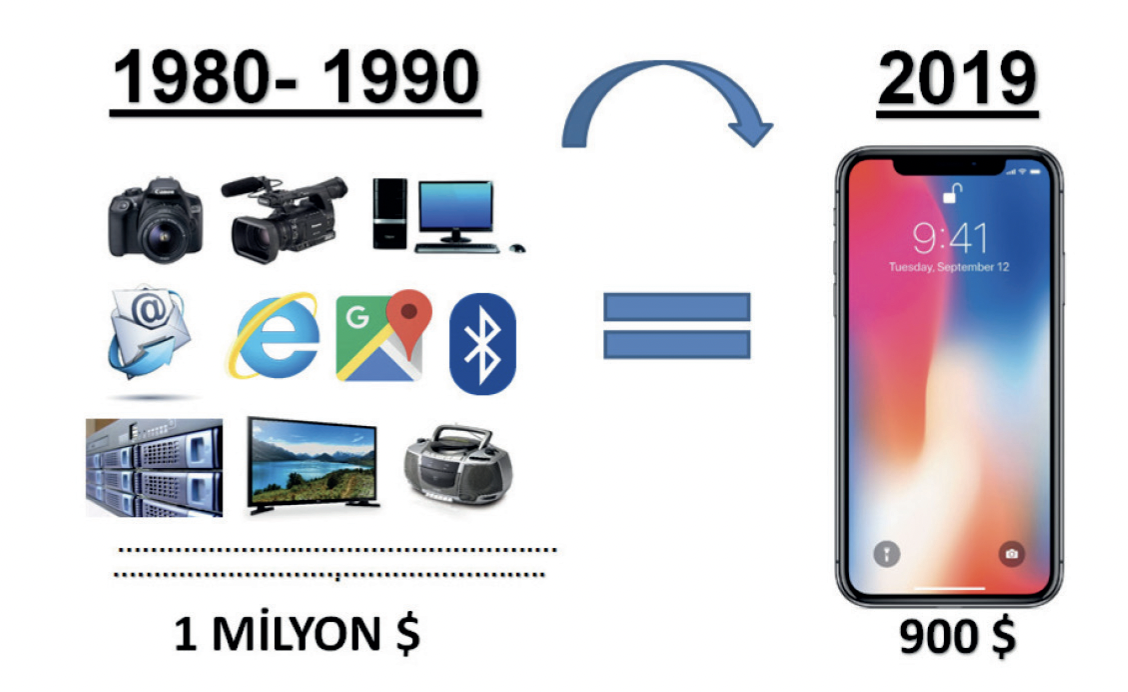
\includegraphics[width=8cm, height=4cm]{ip.png}
  \caption{Sistemler küçülmekte fakat marifetleri büyümektedir \cite{ref5}}
\end{figure}

\newpage
\section{Sonuç}
\begin{multicols}{2}

Dünyada toplumsal ve teknolojik değişim, yüksek bir hızla devam etmektedir.
Dijital dünyanın iş modellerini yükseltebileceği ve işletmelerin yeni ve sürdürülebilir gelir kaynakları bulmak için radikal keşiflere açık olması ve kendilerini rutin
düşünme ve davranıştan koparmaya hazır olmaları gerektiği iyi anlaşılmalıdır.
Bu, kesinlikle bazı riskleri de beraberinde getireceğinden süreçler, yeniden tanımlanmalı ve riskten arındırılabilmek için özel tasarımlar geliştirilmelidir. Sağlıklı bir inovasyon ve rekabetçilik stratejisi belirlenmeli ve bu unsurlar kesintisi
olarak özendirilmelidir. Geliştirilen strateji çok dikkatle uygulanmalıdır. Başta
yapay zekâ olmak üzere teknolojik gelişmelere karşı kayıtsız kalınmamalı ve sistem bütününde tüm operasyonların zekileştirilmesi için gayret gösterilmelidir. 

Hiç kuşkusuz, doğru tasarlandığında, kurgulandığında ve hizmete sunulduğunda, Yapay Zekâ; verimliliği artırabilir, maliyetleri düşürebilir, ürün ve hizmetleri daha yaygın bir şekilde kullanılabilir hale getirebilir ve daha fazla doğruluk ve
hassasiyet sağlayabilir. Bu bağlamda, özel işletmeler ve kamu kurumları, Yapay
Zekâ’nın bu potansiyelinden nasıl yararlanabileceklerini ve bunu yapabilmeleri
için personelini nasıl eğiteceklerini planlamalıdır. Özellikle temel araştırmalara
daha fazla yatırım yapılması gerektiğinden, Yapay Zekâ konusunda yapılacak
araştırmalara karar vericilerin de dâhil edilmesi gerekmektedir. Yapay Zekâ’nın
gelecekte en çok eğitim-öğretim süreçlerinde öğretmenlere yardımcı olabileceği
öngörülmekte olup, bu konudaki yatırımlara ve çalışmalara hız ve önem verilmelidir. Şurası açıktır ki, gelecekte dünyada söz sahibi olmayı planlayan toplumlar, Yapay Zekâ’nın geleceğine de yatırım yapmak zorundadır.

Yüz tanıma teknolojisi gibi sadece birkaç yıl önce filmlerde izlediğimiz birçok
konu ve teknoloji artık hayatımızın merkezindedir. Geleceğin teknolojileri, öngörülenden daha hızlı bir şekilde gerçekleşmekte ve hayatımıza girmektedir.
2026 yılında hayatımıza gireceği öngörülen sürücüsüz araç teknolojisi, 2017
itibariyle kullanılmaya başlamıştır. Yapay Zekâ’nın etkilemeyeceği herhangi bir
alan, sektör veya disiplin olması mümkün gözükmemektedir. Ülkelerin ve büyük
şirketlerin yöneticileri de bu hususa vurgu yapmakta ve Yapay Zekâ teknolojilerine yatırım yapmamanın bedelinin çok ağır olacağının altını çizmektedir.
Ülke olarak Yapay Zekâ ve teknolojileri alanında yatırım yapmak ve yetkinlik
kazanabilmek için disiplinlerarası çalışmaya büyük önem vermemiz gerekmekte
olduğu çok açıktır. Toplumsal düzeyde, ilk aşamada algoritma yetkinliğinden
çok veri okuryazarlığı yetkinliğinin artırılması büyük önem arz etmektedir. Profesyonel düzeyde kodlama yeteneğinin artırılması da oldukça mühimdir. Köklerini kültürümüzden ve İslam dünyası filozoflarından alan uygulamalara hâkim
olmak için bizlere düşen görev, bireylerimizin yeteneklerini keşfetmelerini sağlamak ve bu yetenekler üzerine bir bilim ve araştırma toplumu olmak için çok
çalışmaktır.


\newpage
Unutulmamalıdır ki, ‘İnsansız Fabrikalar’ otuz yıl önce de vardı. Bugün de ‘Karanlık Fabrikalar’ var. Veri hep var oldu. Veri aktarımına otuz yıl önce de ihtiyaç
vardı. Bugün de var. Veri aktarımı ve depolama geçmişte RS-232 kablosu ile, kaset ile, disket ile CD ile yapılıyordu. Bugün internet ile, intranet ile, flashdisk ile,
ağ üzerinden, bulut üzerinden yapılıyor. Görüldüğü üzere; konular, problemler
ve ihtiyaçlar aslında değişmiyor. Değişen ve gelişen şey aslında teknolojinin kendisi! Ve asıl önemli olan da değişen ve gelişen teknolojiye ayak uydurabilmektir.
Tabii, teknolojiyi geliştirmek ve yönlendirmek, ona ayak uydurmaktan çok daha
evladır. Yapay Zekâ konusunda da durum böyledir. İsmi, ister Endüstri 4.0, ister
Toplum 5.0, ister Dijital Çağ, ister Yapay Zekâ Çağı olsun, her ne olursa olsun, bu kavramların, bu yaklaşımların aslında insanın bizatihi kendisini, içindeki
‘insanı’ yeniden keşfedebilmesi için çok büyük fırsatlar sunduğu da çok açıktır.
Kimilerine göre insansı bir robot olarak hayal edilen ‘İnsan 2.0’, kimilerine göre
ise, orijinal ayarlarına dönen insan olarak da tasavvur edilebilir. Eşref-i mahlûkat olan insan, Yapay Zekâ teknolojileri ile yoğurulsa, harmanlansa ve hatta sarsılsa bile, ‘insan’ olarak kalabilmenin çarelerini bulabilecek kadar zekidir. Doğru
stratejiler geliştirildiği takdirde, Yapay Zekâ ve teknolojilerinin toplum hayatını
kolaylaştıracağı, insanlığın sorunlarına çare olacağına olan inancımız da tamdır. 
    
\end{multicols}





\vspace{20pt}
\begin{thebibliography}
    .\bibitem{ref1} \href{https://mbkaya.com/makine-dusunebilir-mi-cahit-arf/}{https://mbkaya.com/makine-dusunebilir-mi-cahit-arf/}

    \bibitem{ref2} \href{https://slate.com/technology/2022/01/ibm-watson-health-failure-artificial-intelligence.html}{https://slate.com/technology/2022/01/ibm-watson-health-failure-artificial-intelligence.html}

    \bibitem{ref3}
    \href{https://incubator.ucf.edu/what-is-artificial-intelligence-ai-and-why-people-should-learn-about-it/}
    {https://incubator.ucf.edu/what-is-artificial-intelligence-ai-and-why-people-should-learn-about-it/}

    \bibitem{ref4} \href{https://mbkaya.com/makine-dusunebilir-mi-cahit-arf/}{https://mbkaya.com/makine-dusunebilir-mi-cahit-arf/}

    \bibitem{ref5} \href{https://papatyabilim.com.tr/cagdas_endustri_muhendisligi.html/}{https://papatyabilim.com.tr/cagdas_Endustri_Muhendislig .html}


\end{thebibliography}

\end{document}
